\documentclass[a4paper,12pt]{article}   % papír A4, písmo 12 bodu
\usepackage[utf8x]{inputenc}            %kodovaní UTF-8
\usepackage{ucs}                        %kodovani unicode
\usepackage[czech]{babel}               %podpora cestiny
\usepackage[T1]{fontenc}                %pouzij variantu pisma T1 (hacky, carky)
\usepackage[left=2.5cm,right=1.5cm,top=2.5cm,bottom=2.5cm]{geometry} %okraje stranky
\usepackage{amsmath,amsfonts,amssymb}   %podpora matematiky
\usepackage{gensymb,marvosym}           %symboly celsius (\celsius) apod.
%\usepackage{mathptmx}                   %font Times New Roman s~podporou matematiky
\usepackage{times}                      %font Times New Roman (matematika pismem Computer Modern) 
\usepackage{parskip}                    %mezera mezi odstavci
%\usepackage[document]{ragged2e}         %text zarovany vlevo
\usepackage[none]{hyphenat} \sloppy     %slova nedelit a~nepretekat
\usepackage{titlesec}
\setcounter{secnumdepth}{4}
\clubpenalty 10000                      %kontrolovat sirotky
\widowpenalty 10000                     %kontrolovat vdovy
\usepackage{setspace} \onehalfspacing   %podpora pro zmenu radkovani + radkovani 1,5
\usepackage{enumerate}                  %podpora pro zmenu cislovani
\usepackage{parskip}
\usepackage{fancyhdr}                   %vlastni zahlavi a~zapati
\usepackage{graphicx}                   %podpora grafiky
\graphicspath{{materialy/}}                   %vychozi adresar s~obrazky
\usepackage{caption}
\usepackage{subcaption}
\usepackage{siunitx}
\usepackage{MnSymbol,wasysym}
\usepackage[shortlabels]{enumitem}
\usepackage{amsmath}
\usepackage{halloweenmath}

%\usepackage{pgfplots}


%\usepackage[table,xcdraw]{xcolor}

        %%%%%%%--prostredi pro vkladani grafu ---%%%%%%%%%%
\usepackage{float}

\usepackage{url}
\usepackage[unicode]{hyperref}
\usepackage{mhchem}
        %%%%%%%--prostredi pro vkladani grafu ---%%%%%%%%%%

\titleclass{\subsubsubsection}{straight}[\subsection]
\newcounter{subsubsubsection}[subsubsection]
\renewcommand\thesubsubsubsection{\thesubsubsection.\arabic{subsubsubsection}}
\renewcommand\theparagraph{\thesubsubsubsection.\arabic{paragraph}} % optional; useful if paragraphs are to be numbered

\titleformat{\subsubsubsection}
  {\normalfont\normalsize\bfseries}{\thesubsubsubsection}{1em}{}
\titlespacing*{\subsubsubsection}
{0pt}{3.25ex plus 1ex minus .2ex}{1.5ex plus .2ex}

\makeatletter
\renewcommand\paragraph{\@startsection{paragraph}{5}{\z@}%
  {3.25ex \@plus1ex \@minus.2ex}%
  {-1em}%
  {\normalfont\normalsize\bfseries}}
\renewcommand\subparagraph{\@startsection{subparagraph}{6}{\parindent}%
  {3.25ex \@plus1ex \@minus .2ex}%
  {-1em}%
  {\normalfont\normalsize\bfseries}}
\def\toclevel@subsubsubsection{4}
\def\toclevel@paragraph{5}
\def\toclevel@paragraph{6}
\def\l@subsubsubsection{\@dottedtocline{4}{7em}{4em}}
\def\l@paragraph{\@dottedtocline{5}{10em}{5em}}
\def\l@subparagraph{\@dottedtocline{6}{14em}{6em}}
\makeatother

\setcounter{secnumdepth}{4}
\setcounter{tocdepth}{4}
\usepackage{gensymb}

\usepackage{amsmath}

\setlist[enumerate]{itemsep=0mm}


%------------------------------ KONEC PREAMBULE ---------------------------------


\begin{document}
\newfloat{schema}{htbp}{schema}\floatname{schema}{Schéma}
\newfloat{graf}{htbp}{graf}\floatname{graf}{Graf}

\begin{titlepage}


    \begin{center}
        \vspace*{1cm}
            
        \Huge
        \textbf{VLIV TVARU KŘIVKY NA ÚDAJ MĚŘICÍHO PŘÍSTROJE}
            
        \vspace{0.5cm}
        \LARGE
        
            
        \vspace{1.5cm}
            
        \textbf{Jakub Dvořák}
            
        \vfill
            
        
            
        \vspace{0.8cm}
            
        

        \Large
            

        4.10.2020\\
        \vspace*{.5cm}
        
\includegraphics[width=.4\textwidth]{logo-cvut-fee.png}\\
        
            
    \end{center}
\end{titlepage}

\setcounter{page}{0} %cislo strany
\pagestyle{empty} %stranku necislovat

\newpage
\section{Úkol měření}
\label{zadani}
\begin{enumerate}
    \item Změřte napětí na zátěži, jejíž výkon je regulován obvodem s triakem pro úhel sepnutí $\alpha$ přibližně 0\,\textdegree, 45\,\textdegree a~90\,\textdegree~předloženými číslicovými multimetry $\textrm{V}_1$ až $\textrm{V}_4$.
    \item Průběh napětí sledujte na osciloskopu (osciloskop připojte na výstup odporového děliče).
    \item Určete, které z multimetrů měří správně efektivní hodnotu, a~určete relativní chybu metody měření efektivní hodnoty u ostatních.
    \item Z údaje multimetrů, které to umožňují, určete aritmetickou střední hodnotu měřeného průběhu.
    \item Pro úhel sepnutí $\alpha\,=\,90$\,\textdegree~určete aritmetickou střední hodnotu a~efektivní hodnotu napětí rovněž výpočtem z definic. Vypočtené hodnoty srovnejte s naměřenými a~v případě jejich rozdílu analyzujte možné příčiny.
\end{enumerate}

\section{Schéma zapojení}
\begin{schema}
    \centering
    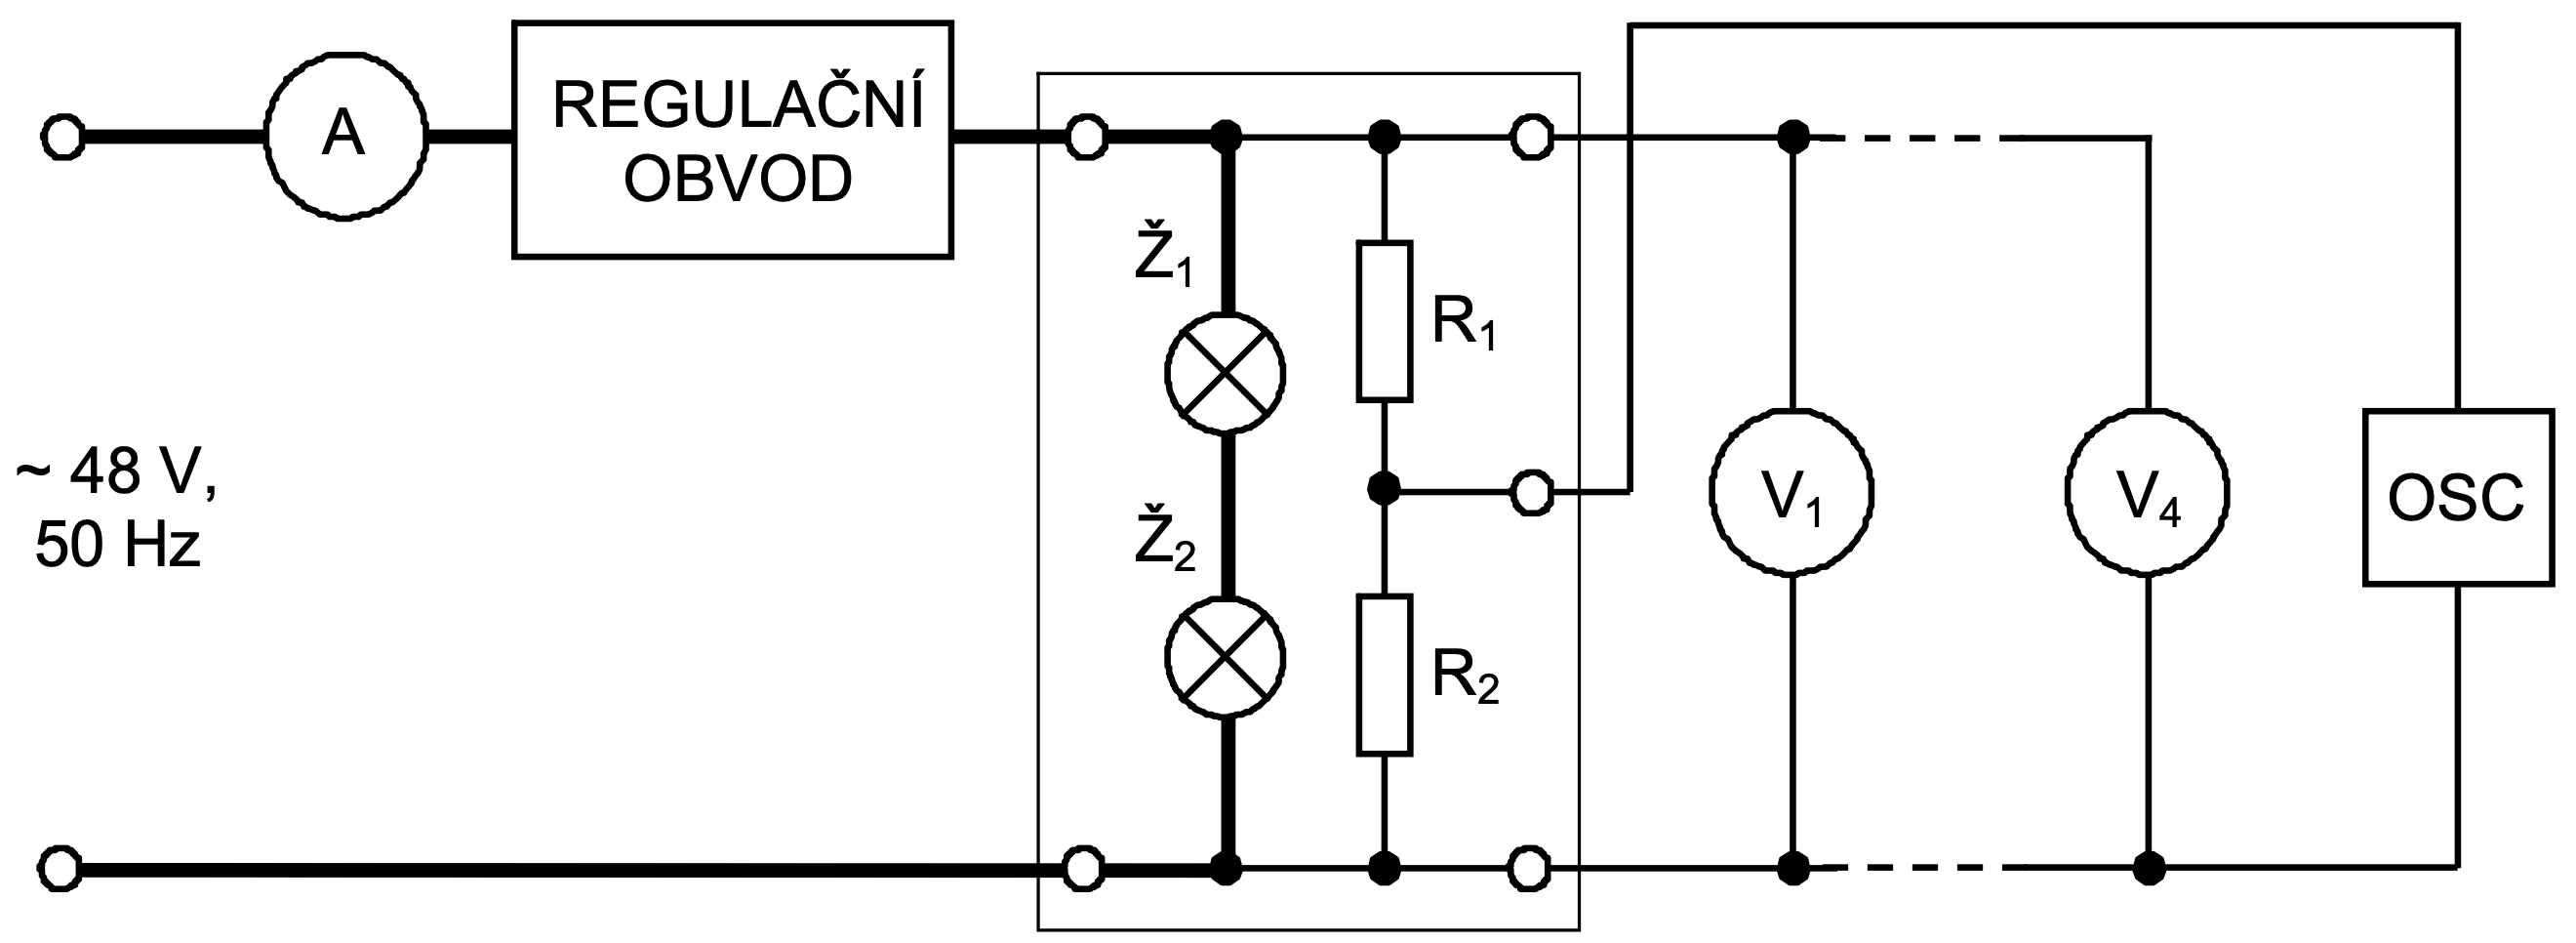
\includegraphics[width=.8\textwidth]{schema_zapojeni.png}
    \caption{Zapojení měřícího obvodu \cite{navod}}
    \label{sch:zapojeni}
\end{schema}

\begin{graf}
    \centering
    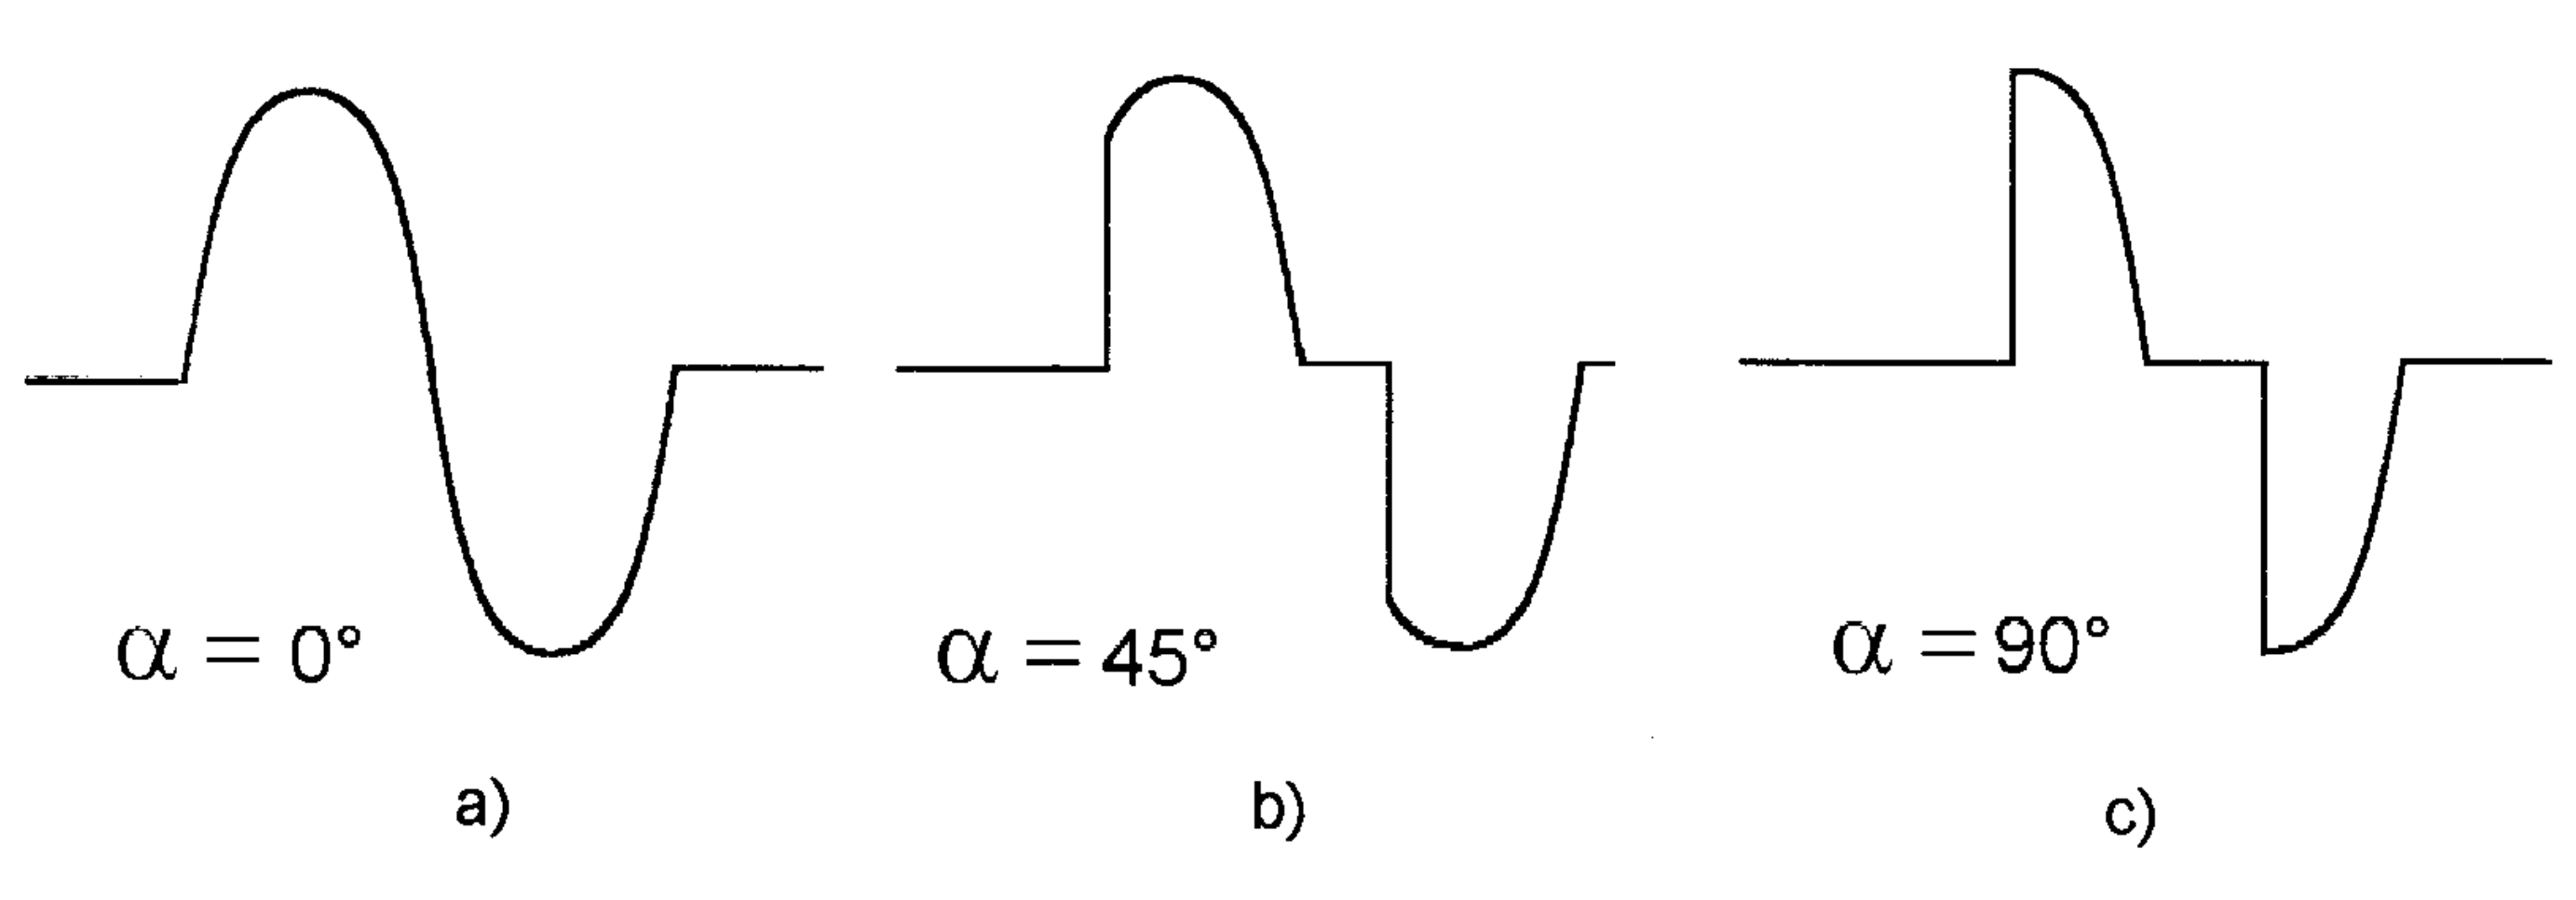
\includegraphics[width=.7\textwidth]{vlny.png}
    \caption{Průběhy měřených napětí \cite{navod}}
    \label{graf:prubehy}
\end{graf}

\section{Seznam použitých přístrojů}
\begin{itemize}
    \item Ampérmetr A
    \item Přípravek se dvěma žárovkami $\textrm{Ž}_1$, $\textrm{Ž}_2$ a~odporovým děličem $\textrm{R}_1$, $\textrm{R}_2$
    \item Ruční multimetr MY64 $\textrm{V}_1$
    \item Stolní multimetr HP 34401 A~$\textrm{V}_2$
    \item Ruční multimetr Summit 45 $\textrm{V}_3$
    \item Ručičkový multimetr TVT-321 $\textrm{V}_4$
    \item Regulační obvod pro regulaci průběhu proudu
\end{itemize}

\section{Teoretický úvod}
Při měření střídavého napětí se využívají dva způsoby, jak zobrazit relevantní hodnotu tj. \textit{střední kvadratickou} (dále jen RMS z anglického \textit{\textbf{R}oot \textbf{M}ean \textbf{S}quare}). V levnějších multimetrech najdeme obvykle precizní usměrňovač tvořený z operačních zesilovačů. Na výstupu dostaneme aritmetickou střední hodnotu a~pro přepočet na RMS se použije koeficient 1,11. Aritmetická hodnota lze spočítat pomocí rovnice~\ref{rce:aritm}. Ve dražších multimetrech je k nalezení dedikovaný RMS převodník, příkladem nechť je AD636 od firmy Analog Devices \cite{datasheet_graf}. Díky RMS převodníku dostaneme skutečnou RMS hodnotu také při neharmonických průbězích napětí. Pro obecnou funkci napětí lze použít rovnice \ref{rce:rms}. 
\begin{equation}
    \
\end{equation}

Efektivní hodnota napětí se při přepočtu na výkon dá použít pro popis tepelného výkonu, jestliže by bylo zařízení napájeno stejnosměrným napětím. Naproti tomu střední aritmetická hodnota odpovídá přenesenému náboji.

\begin{equation}
    U_{\text{ef}}={\sqrt {{1 \over {T}}{\int _{0}^{T}{u^{2}(t)}\,dt}}}
    \label{rce:rms}
\end{equation}

\begin{equation}
    U_{sar}=\frac{1}{T}\int_0^T \lvert u(t)\rvert\,dt~=~ U_{sar}=\frac{2}{T}\int_0^{\frac{T}{2}} \lvert u(t)\rvert\,dt
    \label{rce:aritm}
\end{equation}

Pro sinusový průběh můžeme integrál z rovnice \ref{rce:aritm} vypočítat a~dostaneme
\begin{equation}
    U_{sar,\alpha} = \frac{U_m}{\pi}[-cos\,x]^\pi_\alpha
\end{equation}
a pro efektivní
\begin{equation}
    U_{ef, \alpha}=\frac{U_m}{\sqrt{\pi}} \sqrt{\int_{\alpha}^{\pi} \frac{1-cos2x}{2}\,dx}
\end{equation}

Střední aritmetické a~střední kvadratické hodnoty napětí v závislosti na úhlu sepnutí jsou v tabulce~\ref{tab:calc_hodnoty}.
\begin{table}[h!]
    \centering
    \begin{tabular}{|c|c|c|c|}
        \hline
        &$\alpha=0~\degree$ &$\alpha=45~\degree$    & $\alpha=90~\degree$   \\\hline\hline
        \rule{0pt}{2.5ex}$U_{sar}$  & $2\cdot \frac{U_m}{\pi}$  & $\frac{U_m}{\pi}\cdot\frac{2+\sqrt{2}}{2}$    & $\frac{U_m}{\pi}$ \\[.9ex]\hline
        \rule{0pt}{3.5ex}$U_{ef}$   & $\frac{U_m}{\sqrt{2}}$ & $\frac{1}{2}\sqrt{\frac{2+3\pi}{2\pi}}U_m$ & $\frac{U_m}{2}$ \\[.9ex]\hline
    \end{tabular}
    \caption{Střední aritmetická a~efektivní hodnota v závislosti na úhlu sepnutí}
    \label{tab:calc_hodnoty}
\end{table}


\section{Naměřené hodnoty}
Dle odečtu z videa byly naměřeny hodnoty zobrazené v tabulce \ref{tab:hodnoty}.
\begin{table}[h!]
    \centering
    \begin{tabular}{|c|c|c|c|c|}
    \hline
        \rule{0pt}{2.5ex} Úhel sepnutí & MY64 $\frac{U}{V}$ & HP 34401 a~$\frac{U}{V}$ & Summit 45 $\frac{U}{V}$ & TVT-321 $\frac{U}{V}$\\[.7ex]\hline\hline
        0~\textdegree  & 50,6 & 50,431 & 49,5  & 50  \\\hline
        45~\textdegree & 48,2 & 49,55  & 46,3  & 47,8\\\hline
        90~\textdegree & 32,5 & 39,530 & 30,64 & 30  \\\hline
    \end{tabular}
    \caption{Naměřené hodnoty}
    \label{tab:hodnoty}
\end{table}

\section{Zpracování naměřených hodnot}

Pro přepočet ze střední kvadratické na maximální napětí $U_m$ využijeme vzorce
\begin{equation*}
    \begin{split}
    U_m&=U_{ef}\cdot\sqrt{2} \textrm{~pro~} 0\,\degree,\\
    U_m&=U_{ef}\cdot2\sqrt{\frac{2\pi}{2+3\pi}} \textrm{~pro~}45\,\degree,\\
    U_m&=U_{ef}\cdot2 \textrm{~pro~}90\,\degree,\\
    \end{split}
\end{equation*}
čímž dostaneme tabulku \ref{tab:umax} maximálních napětí, které naměřily různé multimetry pro různé úhly spuštění:
\begin{table}[h!]
    \centering
    \begin{tabular}{|c|c|c|c|c|}
    \hline
     \rule{0pt}{2.5ex} Úhel sepnutí & MY64 $\frac{U_m}{V}$ & HP 34401 a~$\frac{U_m}{V}$ & Summit 45 $\frac{U_m}{V}$ & TVT-321 $\frac{U_m}{V}$\\[.7ex]\hline\hline
    0~\textdegree   &   71,559&	71,320&	70,004&	70,711\\\hline
    45~\textdegree &	35,745&	36,746&	34,336&	35,448\\\hline
    90~\textdegree &	65,000&	79,060&	61,260&	60,000\\\hline
    \end{tabular}
    \caption{Vypočítané hodnoty maximálního napětí $U_m$}
    \label{tab:umax}
\end{table}

Z hodnot $U_m$ pro 0\,\textdegree si poté s použitím vzorců z tabulky \ref{tab:calc_hodnoty} vypočítáme správná efektivní napětí $U_{ef}$ a~porovnáme s naměřenými hodnotami z tabulky \ref{tab:hodnoty}.

\begin{table}[h!]
    \centering
    \begin{tabular}{|c|c|c|c|c|}
    \hline
     \rule{0pt}{2.5ex} Úhel sepnutí & MY64 $\frac{U_{ef}}{V}$ & HP 34401 a~$\frac{U_{ef}}{V}$ & Summit 45 $\frac{U_{ef}}{V}$ & TVT-321 $\frac{U_{ef}}{V}$\\[.7ex]\hline\hline
    0~\textdegree   &	50,6   	&50,431	&49,5	&50     \\\hline
    45~\textdegree  &	48,246	&48,086	&47,2	&47,675 \\\hline
    90~\textdegree	&   35,779	&35,66	&35	    &35,355 \\\hline
    \end{tabular}
    \caption{Hodnoty $U_{ef}$ spočítané podle $U_{m,0\,\degree}$ z tabulky \ref{tab:umax}}
    \label{tab:ef_vypocitane}
\end{table}

Při porovnání s tabulkou hodnot \ref{tab:hodnoty}, které jsme naměřili je vidět, že při úhlu zapnutí $\alpha = 90\,\degree$ jsou všechna měřená napětí velice odlišná od vypočítaných napětí. Nejrelevantnější způsob popisu je pomocí \textit{relativní chyby měření}

Pro relativní chybu měření nejdříve potřebujeme znát absolutní chybu $\delta_M$ Ta se vypočítá jako $\delta_X=X_{M}-X_{S}$, kde $X_M$ je měřená hodnota a $X_S$ je skutečná hodnota. Relativní chybu následně vypočítáme jako $\Delta_X=\delta_X / X_{M}$. Měřená hodnota byla brána z tabulky \ref{tab:hodnoty} a skutečná hodnota z tabulky \ref{tab:ef_vypocitane}. Obě pro úhel sepnutí 90\,\textdegree. Hodnoty jednotlivých absolutních a~relativních chyb jsou v tabulce \ref{tab:relchyba}.

\begin{table}[h!]
    \centering
    \begin{tabular}{|c|c|c|c|c|l|}
    \hline
     \rule{0pt}{2.5ex}& MY64& HP 34401 A& Summit 45 & TVT-321 & rozměr\\[.7ex]\hline\hline
    Absolutní   &3,28   &3,87	&4,372	&5,355& V\\\hline
    Relativní   &0,101  &0,098	&0,143	&0,179& 1\\\hline
    \end{tabular}
    \caption{Absolutní a~relativní chyby měření pro úhel sepnutí $\alpha$ = 90\,\textdegree}
    \label{tab:relchyba}
\end{table}

Pro zjištění střední aritmetické hodnoty využijeme tabulku maximálních napětí \ref{tab:umax}, která má pro každý průběh vypočítané $U_m$ odpovídající měřené hodnotě ${U_{ef}}$. Proto můžeme tuto hodnotu použít spolu se vzorci z tabulky \ref{tab:calc_hodnoty} na spočítání $U_{sar}$. Hodnoty $U_{sar}$ pro jednotlivé průběhy a multimetry jsou zanesené v tabulce \ref{tab:sar}.

\begin{table}[h!]
    \centering
    \begin{tabular}{|c|c|c|c|c|}
    \hline
     \rule{0pt}{2.5ex} Úhel sepnutí & MY64 $\frac{U_{sar}}{V}$ & HP 34401 a~$\frac{U_{sar}}{V}$ & Summit 45 $\frac{U_{sar}}{V}$ & TVT-321 $\frac{U_{sar}}{V}$\\[.7ex]\hline\hline
    0~\textdegree	&45,55	&45,40	&44,57	&45,02\\\hline
    45~\textdegree	&26,19	&26,92	&25,16	&25,97\\\hline
    90~\textdegree	&20,69	&25,17	&19,5	&19,1\\\hline
    \end{tabular}
    \caption{Hodnoty $U_{sar}$ spočítané podle $U_{m,0\,\degree}$ z tabulky \ref{tab:umax}}
    \label{tab:sar}
\end{table}


\section{Závěrečné vyhodnocení}
Ověřili jsme, že úhel sepnutí sinusového průběhu má vliv na efektivní hodnotu napětí. Tohoto je využito například ve stmívačích světel, díky čemuž jde regulovat výkon, který jde od žárovky. Jelikož spínací triak pouze vede/nevede, netvoří se na něm takové výkonové ztráty, jako například na tranzistoru, který by reguloval stejnosměrný proud.

Multimetry, které jsem využili, neměřily ani v jednom případě správnou efektivní hodnotu a jejich relativní chyba měření se pohybovala od 0,098 do 0,179, což je velice špatný výsledek. A to i u multimetru HP, který by podle \textit{datasheetu} měl mít funkci \textit{True RMS} \cite{datasheet_multimetry}.


%--- LITERATURA a~ZDROJE (povinne) ---
\clearpage
\renewcommand{\refname}{Seznam použité literatury a~zdrojů informací} 
%\section*{Seznam použité literatury a~zdrojů informací}
\phantomsection %pridej odkaz do PDF zalozek
\addcontentsline{toc}{section}{Seznam použité literatury a~zdrojů informací}

\begin{thebibliography}{99}

%----------------------------------------------------
\subsection*{Seznam použitých internetových zdrojů}
    \bibitem{navod} Návod k laboratorní úloze
    \bibitem{datasheet_graf} \url{https://www.analog.com/media/en/technical-documentation/data-sheets/AD636.pdf}
    \bibitem{datasheet_multimetry} \url{https://moodle.fel.cvut.cz/pluginfile.php/267148/mod_resource/content/1/Devices%20Data%20Sheets.pdf}
    
\end{thebibliography}




\end{document}